\begin{frame}
\frametitle{}
\begin{center}
{\fontsize{49}{90}\selectfont
{\color{title} Getting Started}}
\end{center}

\begin{itemize}
\item Running Python and loading NetworkX
\item Creating a Graph, adding nodes and edges
\item Finding what is in NetworkX
\item Interacting with NetworkX graphs
\item Graph generators and operators
\item Basic analysis of graphs
\end{itemize}
\end{frame}

\begin{frame}
\frametitle{Running Python and loading NetworkX}
IPython Command line
\centerline{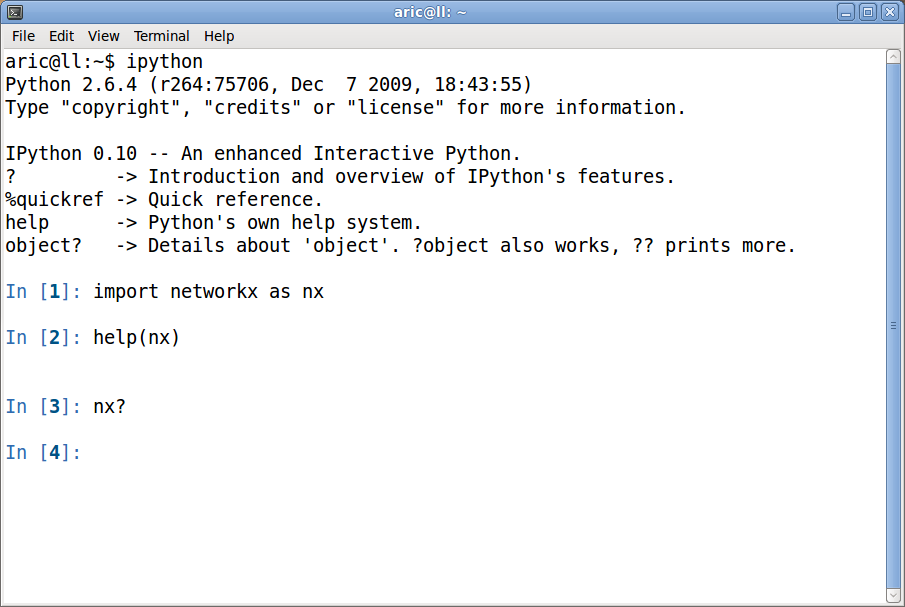
\includegraphics[width=4.0in]{nx-ipython}}
No GUI \footnotesize{http://www.cryptonomicon.com/beginning.html}
\end{frame}

\begin{frame}
\frametitle{Command line vs executing file}
You can type commands interactively or put them in a file and run them.
\centerline{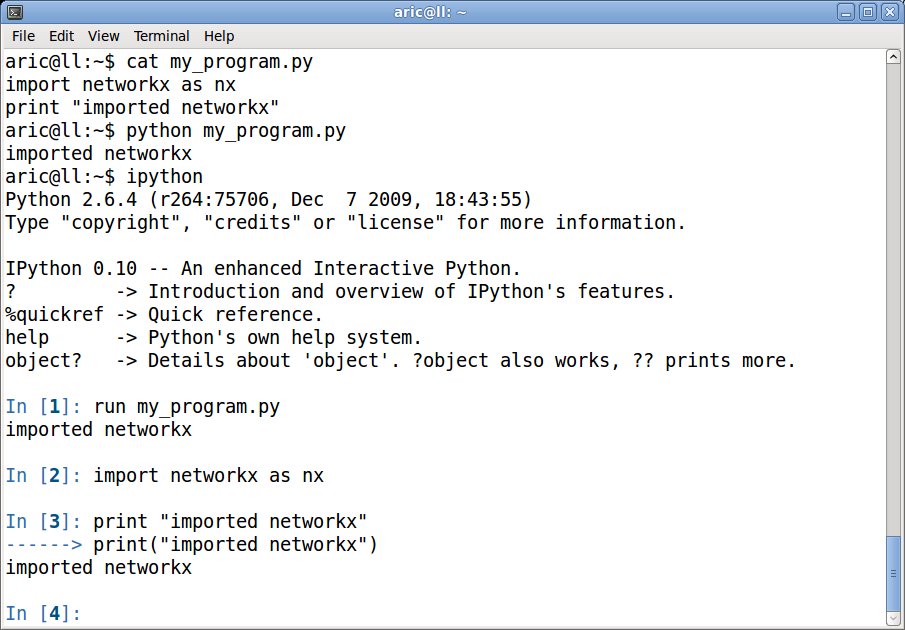
\includegraphics[width=4.0in]{ipython-import}}
\end{frame}

\begin{frame}
\frametitle{Creating a graph}

The basic $Graph$ object is used to hold the network information.

Create an empty graph (no nodes or edges):

\begin{block}{}
\lstinputlisting[firstline=1,lastline=4]{code/build_graph.py.doctest}
\end{block}

The graph G can be grown in several ways.

NetworkX includes many graph generator functions
and facilities to read and write graphs in many formats.
\end{frame}


\begin{frame}[fragile]
\frametitle{Adding nodes}

\begin{block}{}
\lstinputlisting[firstline=5,lastline=17]{code/build_graph.py.doctest}
\end{block}

Nodes can be any hashable object such as strings,
numbers, files, functions, and more.

\end{frame}



\begin{frame}[fragile]

G can also be grown by adding edges.

\begin{block}{}
\lstinputlisting[firstline=18,lastline=35]{code/build_graph.py.doctest}

\end{block}

If the nodes do not already exist they are automatically added to the graph.

You can demolish the graph similarly with
\begin{verbatim}
G.remove_node, G.remove_nodes_from,
G.remove_edge, G.remove_edges_from.
\end{verbatim}

\end{frame}

\begin{frame}
\Large
\begin{itemize}

\item How do I find out the names of the methods like add\_edge?

\item How do I see what is in my graph?

\end{itemize}
\end{frame}

\begin{frame}
\frametitle{What's in NetworkX?}
\centerline{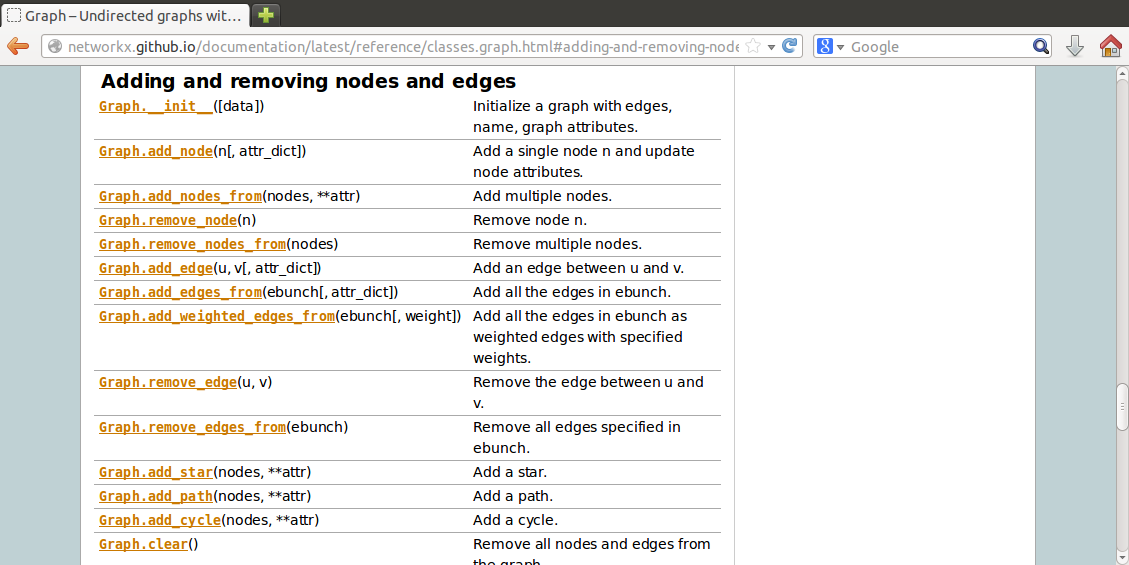
\includegraphics[width=1.0\columnwidth]{nx-doc-add}}
\end{frame}

\begin{frame}
\frametitle{What's in NetworkX?}
\centerline{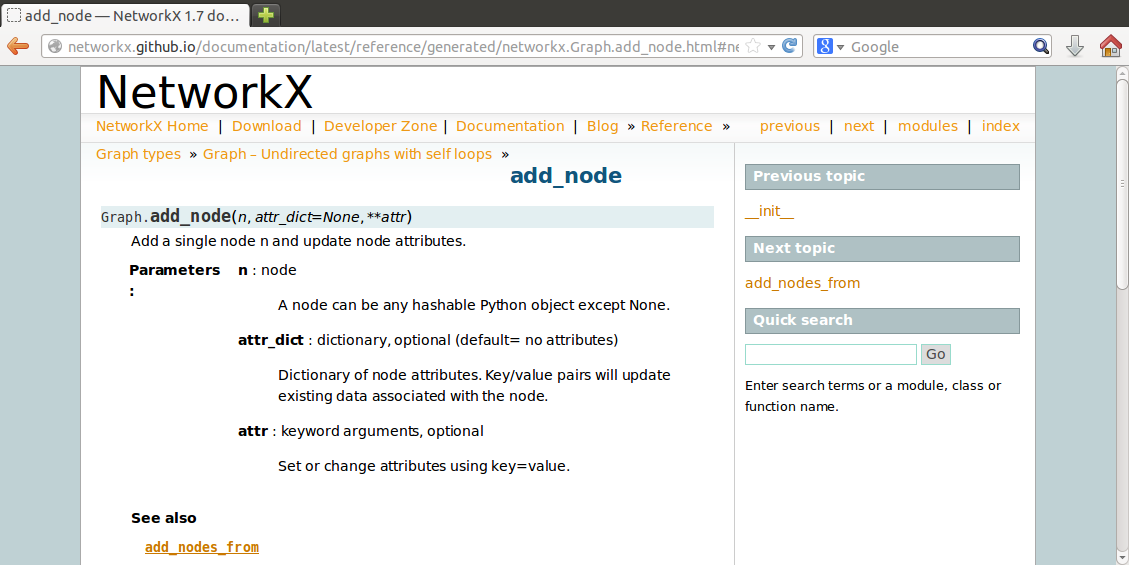
\includegraphics[width=1.0\columnwidth]{nx-doc-add-1}}
\end{frame}

\begin{frame}
\frametitle{What's in Networkx?}
\centerline{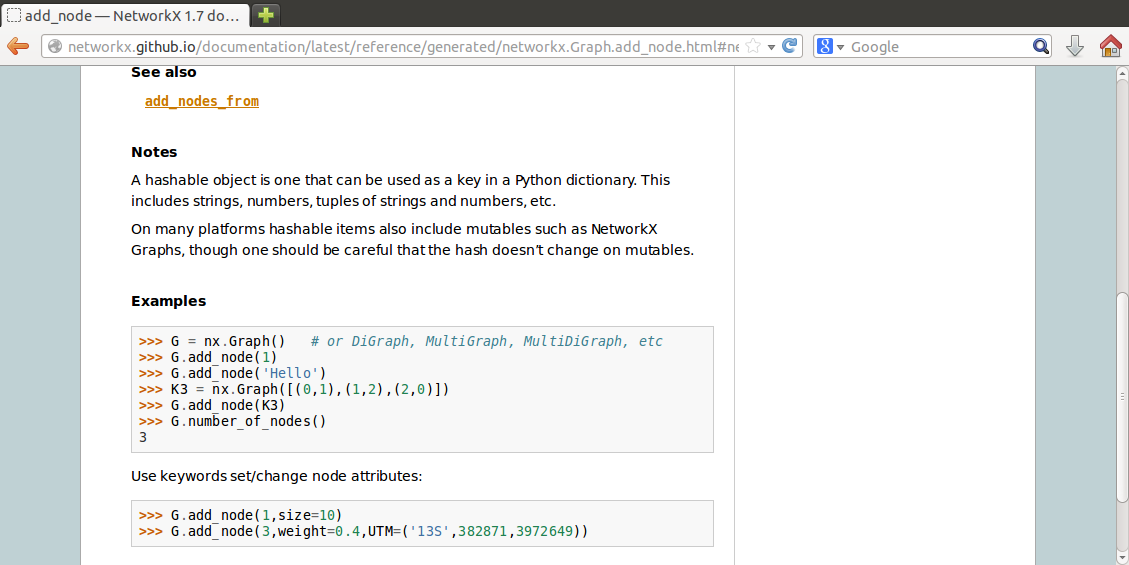
\includegraphics[width=1.0\columnwidth]{nx-doc-add-2}}
\end{frame}

\begin{frame}
\frametitle{What's in Networkx?}
\centerline{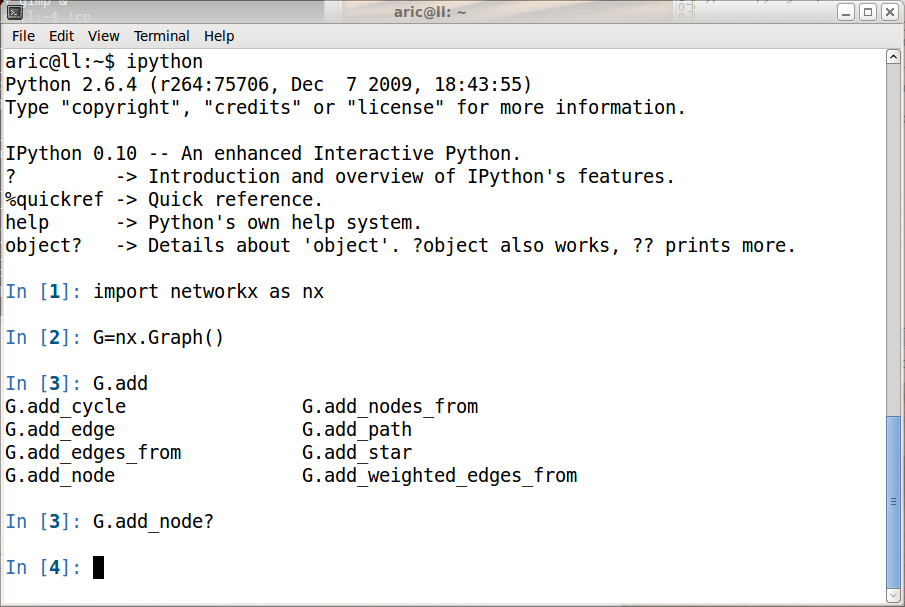
\includegraphics[width=4.0in]{nx-ipython-tab}}
\end{frame}

\begin{frame}
\frametitle{What's in Networkx?}
\centerline{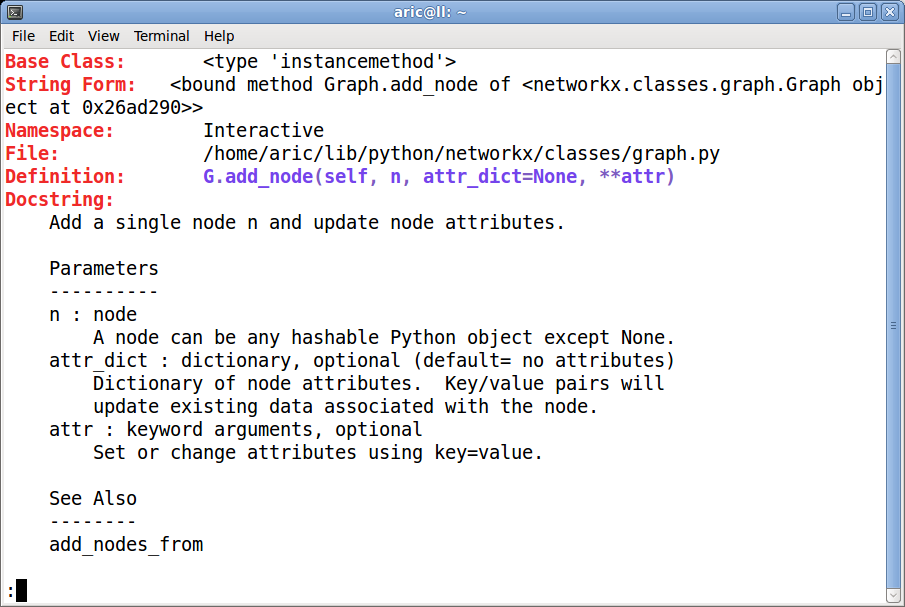
\includegraphics[width=4.0in]{nx-ipython-tab-add}}
\end{frame}


\begin{frame}
\frametitle{What's in Networkx?}
\centerline{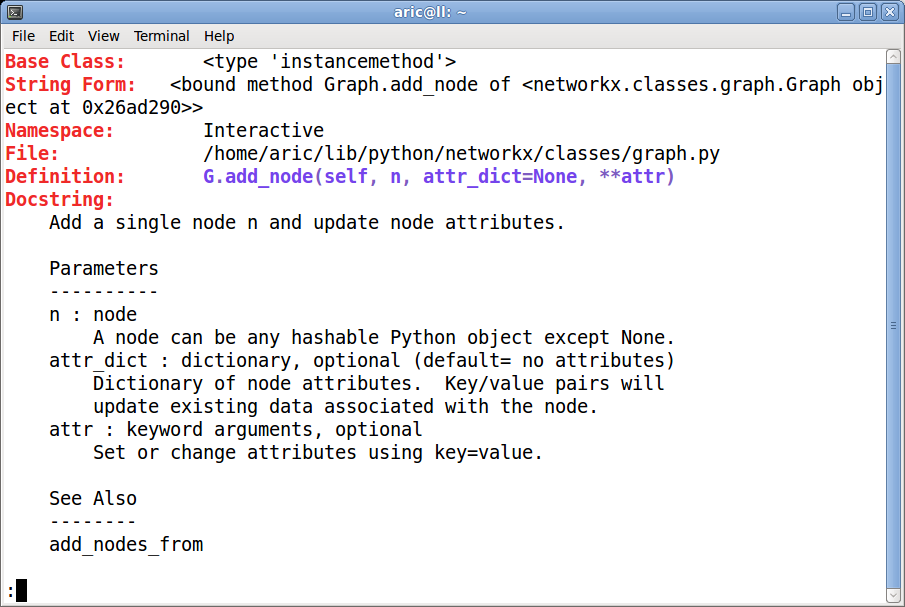
\includegraphics[width=4.0in]{nx-ipython-tab-add}}
Demo
\end{frame}

\begin{frame}[fragile]
\frametitle{Adding attributes to graphs, nodes, and edges}

\begin{columns}
\begin{column}{0.3\textwidth}

(Almost) any Python object is allowed as graph, node, and edge data.
\begin{itemize}
\item number
\item string
\item image
\item IP address
\item email address
\end{itemize}
\end{column}

\begin{column}{0.7\textwidth}
\centerline{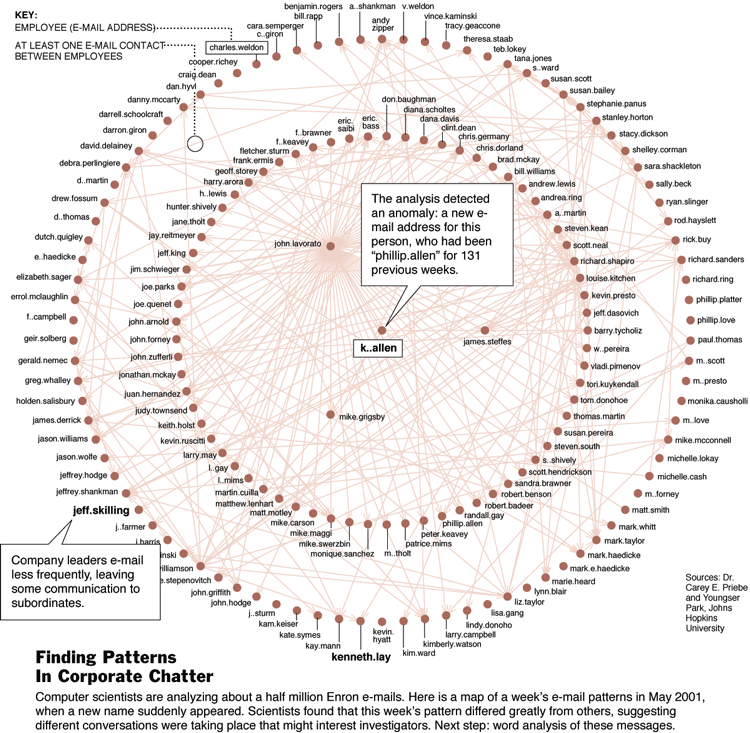
\includegraphics[width=1.0\columnwidth]{enron}}
\end{column}

\end{columns}

\end{frame}


\begin{frame}[fragile]
\frametitle{Graph attributes}
\lstinputlisting[firstline=1,lastline=12]{code/attributes.py.doctest}

\end{frame}



\begin{frame}[fragile]
\frametitle{Node attributes}
\lstinputlisting[firstline=13,lastline=25]{code/attributes.py.doctest}

\end{frame}

\begin{frame}[fragile]
\frametitle{Edge attributes}
\lstinputlisting[firstline=27,lastline=45]{code/attributes.py.doctest}

\end{frame}

\begin{frame}[fragile]
\frametitle{Weighted graph example}
\begin{columns}
\begin{column}{0.7\textwidth}
The special attribute 'weight'
holds values used by algorithms requiring weighted edges.

\end{column}

\begin{column}{0.3\textwidth}
\centerline{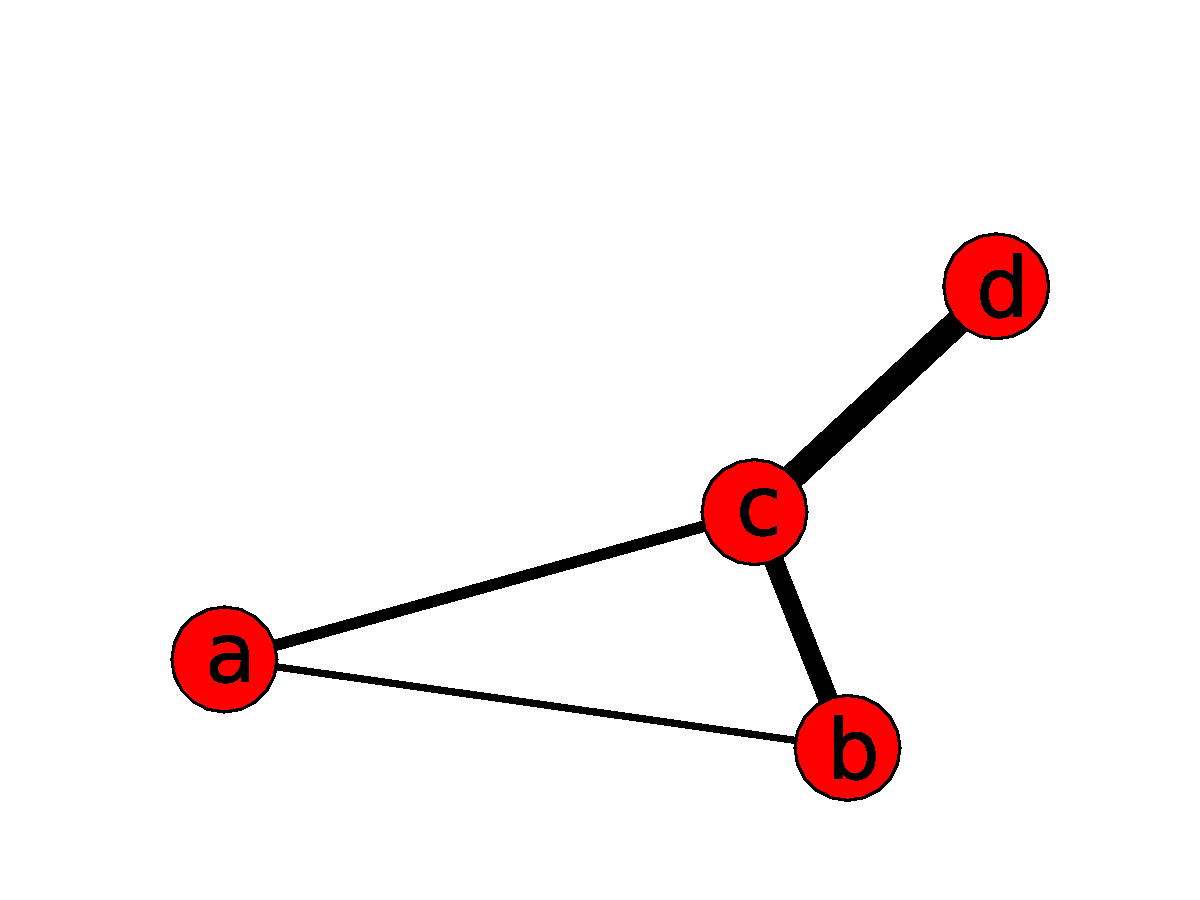
\includegraphics[width=1.4\columnwidth]{dijkstra}}
\end{column}
\end{columns}

\begin{block}{}
Use Dijkstra's algorithm to find the shortest path:


\lstinputlisting{code/dijkstra.py.doctest}
\end{block}

\end{frame}

\begin{frame}[fragile]
\frametitle{More ways to build graphs: operators and generators}

Applying classic graph operations

\begin{description}

\item[subgraph(G, nbunch)]      - induce subgraph of G on nodes in nbunch
\item[union(G1, G2)] - graph union
\item[disjoint\_union(G1, G2)]   - graph union assuming all nodes are different
\item[cartesian\_product(G1, G2)] - return Cartesian product graph
\item[compose(G1,G2)]           - combine graphs identifying nodes common to both
\item[complement(G)]            - graph complement
\item[create\_empty\_copy(G)]     - return an empty copy of the same graph class
\item[convert\_to\_undirected(G)] - return an undirected representation of G
\item[convert\_to\_directed(G)]   - return a directed representation of G
\end{description}

\end{frame}

\begin{frame}
\frametitle{Call a graph generator}

\lstinputlisting[firstline=2]{code/generators.py.doctest}
\end{frame}

\begin{frame}[fragile]
\frametitle{Basic analysis of graphs}

\lstinputlisting[firstline=2]{code/analysis.py.doctest}


\end{frame}
